WaveNet adalah jaringan saraf dalam untuk menghasilkan audio mentah. Itu dibuat oleh para peneliti di perusahaan AI yang berbasis di London, DeepMind . Teknik yang diuraikan dalam makalah pada bulan September 2016, mampu menghasilkan suara mirip manusia yang terdengar relatif realistis dengan secara langsung memodelkan bentuk gelombang menggunakan metode jaringan saraf yang dilatih dengan rekaman ucapan nyata. Pengujian dengan bahasa Inggris dan Mandarin AS dilaporkan menunjukkan bahwa sistem tersebut mengungguli sistem text-to-speech (TTS) terbaik yang ada di Google, meskipun pada 2016 sintesis text-to-speechnya masih kurang meyakinkan daripada ucapan manusia yang sebenarnya. Kemampuan WaveNet untuk menghasilkan bentuk gelombang mentah berarti dapat memodelkan semua jenis audio, termasuk musik\cite{DBLP:journals/corr/OordDZSVGKSK16}.
Menghasilkan ucapan dari teks adalah tugas yang semakin umum berkat popularitas perangkat lunak seperti Siri Apple, Cortana Microsoft, Amazon Alexa, dan Asisten Google.

Sebagian besar sistem tersebut menggunakan variasi teknik yang melibatkan fragmen suara yang digabungkan bersama untuk membentuk suara dan kata yang dapat dikenali, yang paling umum disebut TTS gabungan. Ini terdiri dari perpustakaan besar fragmen pidato, direkam dari satu pembicara yang kemudian digabungkan untuk menghasilkan kata-kata dan suara yang lengkap. Hasilnya terdengar tidak wajar, dengan irama dan nada yang aneh. Ketergantungan pada perpustakaan yang direkam juga membuat sulit untuk memodifikasi atau mengubah suara.

Teknik lain, yang dikenal sebagai TTS parametrik, menggunakan model matematika untuk menciptakan kembali suara yang kemudian dirangkai menjadi kata dan kalimat. Informasi yang diperlukan untuk menghasilkan suara disimpan dalam parameter model. Karakteristik pidato keluaran dikendalikan melalui input ke model, sedangkan pidato biasanya dibuat menggunakan synthesizer suara yang dikenal sebagai vocoder. Ini juga dapat menghasilkan audio yang terdengar tidak wajar.

WaveNet adalah jenis feedforward neural network yang dikenal sebagai deep convolutional neural network (CNN). Di WaveNet, CNN mengambil sinyal mentah sebagai input dan mensintesis output satu sampel pada satu waktu. Ia melakukannya dengan mengambil sampel dari distribusi softmax (yaitu kategorikal ) dari nilai sinyal yang dikodekan menggunakan transformasi -law companding dan dikuantisasi ke 256 nilai yang mungkin.

Menurut makalah penelitian DeepMind September 2016 Original WaveNet: A Generative Model for Raw Audio, jaringan tersebut diberi makan bentuk gelombang nyata dari pidato dalam bahasa Inggris dan Mandarin. Saat ini melewati jaringan, ia mempelajari seperangkat aturan untuk menggambarkan bagaimana bentuk gelombang audio berkembang dari waktu ke waktu. Jaringan terlatih kemudian dapat digunakan untuk membuat bentuk gelombang seperti ucapan baru pada 16.000 sampel per detik\cite{DBLP:journals/corr/OordDZSVGKSK16}.

WaveNet mampu memodelkan suara yang berbeda secara akurat, dengan aksen dan nada input yang berkorelasi dengan output. Misalnya, jika dilatih dengan bahasa Jerman, ia menghasilkan pidato bahasa Jerman. Kemampuan ini juga berarti bahwa jika WaveNet diberi masukan lain – seperti musik – keluarannya akan berupa musik. Pada saat dirilis, DeepMind menunjukkan bahwa WaveNet dapat menghasilkan bentuk gelombang yang terdengar seperti musik klasik.

Makalah Januari 2019 Pembelajaran representasi ucapan tanpa pengawasan menggunakan autoencoder WaveNet merinci metode untuk berhasil meningkatkan pengenalan otomatis yang tepat dan diskriminasi antara fitur dinamis dan statis untuk "pertukaran konten", terutama termasuk menukar suara pada rekaman audio yang ada, di untuk membuatnya lebih dapat diandalkan. Makalah tindak lanjut lainnya, Sample Efficient Adaptive Text-to-Speech, tertanggal September 2018 (revisi terbaru Januari 2019), menyatakan bahwa DeepMind telah berhasil mengurangi jumlah minimum rekaman kehidupan nyata yang diperlukan untuk mengambil sampel suara yang ada melalui WaveNet untuk "hanya beberapa menit data audio" sambil mempertahankan hasil berkualitas tinggi.

Kemampuannya untuk mengkloning suara telah menimbulkan kekhawatiran etis tentang kemampuan WaveNet untuk meniru suara orang hidup dan mati. Menurut artikel BBC 2016 , perusahaan yang mengerjakan teknologi kloning suara serupa (seperti Adobe Voco) bermaksud untuk memasukkan tanda air yang tidak terdengar oleh manusia untuk mencegah pemalsuan, sambil mempertahankan kloning suara yang memuaskan, misalnya, kebutuhan tujuan industri hiburan akan memiliki kompleksitas yang jauh lebih rendah dan menggunakan metode yang berbeda dari yang diperlukan untuk menipu metode pembuktian forensik dan perangkat ID elektronik, sehingga suara alami dan suara yang dikloning untuk tujuan industri hiburan masih dapat dengan mudah dibedakan dengan analisis teknologi.

Pada saat peluncurannya, DeepMind mengatakan bahwa WaveNet membutuhkan terlalu banyak kekuatan pemrosesan komputasi untuk digunakan dalam aplikasi dunia nyata. Pada Oktober 2017, Google mengumumkan peningkatan kinerja 1.000 kali lipat bersama dengan kualitas suara yang lebih baik. WaveNet kemudian digunakan untuk menghasilkan suara Asisten Google untuk bahasa Inggris AS dan Jepang di semua platform Google. Pada bulan November 2017, peneliti DeepMind merilis makalah penelitian yang merinci metode yang diusulkan untuk "menghasilkan sampel ucapan dengan ketelitian tinggi lebih dari 20 kali lebih cepat daripada waktu nyata", yang disebut "Distilasi Kepadatan Probabilitas". Pada konferensi pengembang I/O tahunanpada Mei 2018, diumumkan bahwa suara Asisten Google baru tersedia dan dimungkinkan oleh WaveNet; WaveNet sangat mengurangi jumlah rekaman audio yang diperlukan untuk membuat model suara dengan memodelkan audio mentah dari sampel aktor suara.

\section{Talking Machine}
Mengizinkan orang berkomunikasi dengan mesin adalah impian lama interaksi manusia-komputer. Kemampuan komputer untuk memahami ucapan alami telah mengalami revolusi dalam beberapa tahun terakhir dengan penerapan jaringan saraf dalam (misalnya, Google Voice Search ). Namun, menghasilkan pidato dengan komputer — sebuah proses yang biasanya disebut sebagai sintesis ucapan atau text-to-speech (TTS) — sebagian besar masih didasarkan pada apa yang disebut TTS concatenative , di mana database yang sangat besar dari fragmen pidato pendek direkam dari satu penutur dan kemudian digabungkan kembali untuk membentuk ujaran yang lengkap. Hal ini membuat sulit untuk memodifikasi suara (misalnya beralih ke pembicara yang berbeda, atau mengubah penekanan atau emosi ucapan mereka) tanpa merekam database yang sama sekali baru.

Hal ini menyebabkan permintaan yang besar untuk TTS parametrik , di mana semua informasi yang diperlukan untuk menghasilkan data disimpan dalam parameter model, dan isi serta karakteristik pidato dapat dikontrol melalui input ke model. Sejauh ini, bagaimanapun, TTS parametrik cenderung terdengar kurang alami daripada concatenative. Model parametrik yang ada biasanya menghasilkan sinyal audio dengan melewatkan outputnya melalui algoritma pemrosesan sinyal yang dikenal sebagai vocoder .

WaveNet mengubah paradigma ini dengan secara langsung memodelkan bentuk gelombang mentah dari sinyal audio, satu sampel pada satu waktu. Selain menghasilkan ucapan yang terdengar lebih alami, menggunakan bentuk gelombang mentah berarti WaveNet dapat memodelkan semua jenis audio, termasuk musik.

\section{WaveNet Improving State of The Arts}
Kami melatih WaveNet menggunakan beberapa kumpulan data TTS Google sehingga kami dapat mengevaluasi kinerjanya. Gambar berikut menunjukkan kualitas WaveNets pada skala 1 sampai 5, dibandingkan dengan sistem TTS terbaik Google saat ini ( parametrik  dan  concatenative ), dan dengan ucapan manusia menggunakan  Mean Opinion Scores (MOS) . MOS adalah ukuran standar untuk tes kualitas suara subjektif, dan diperoleh dalam tes buta dengan subjek manusia (dari lebih dari 500 peringkat pada 100 kalimat tes). Seperti yang dapat kita lihat, WaveNets mengurangi kesenjangan antara keadaan seni dan kinerja tingkat manusia lebih dari 50\% untuk bahasa Inggris AS dan Mandarin.

Untuk bahasa Cina dan Inggris, sistem TTS Google saat ini dianggap sebagai yang terbaik di seluruh dunia, jadi meningkatkan keduanya dengan satu model merupakan pencapaian besar.

\begin{figure}[H]
        \centerline{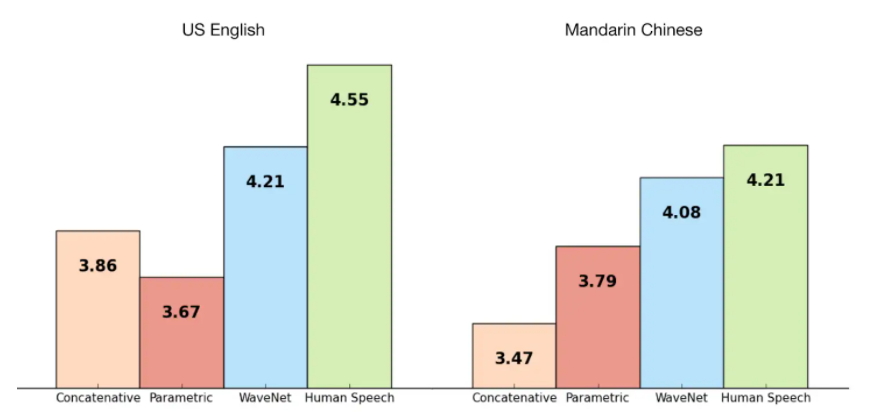
\includegraphics[scale=.5]{figures/wavenet}}
        \caption{Perbandingan WaveNet dengan Model Lain}
		\label{wavenet}
\end{figure}
Untuk menarik perbandingan antara WaveNet dan pendekatan sintesis ucapan yang ada, tes Subjektif 5-skala Mean Opinion Score (MOS) dilakukan. Dalam tes MOS, subjek (manusia) disajikan dengan sampel ucapan yang dihasilkan dari salah satu sistem sintesis ucapan dan diminta untuk menilai kealamian sampel ucapan dalam skor skala lima poin (1: Buruk, 2: Buruk, 3 : Cukup, 4: Baik, 5: Sangat Baik).

Terlihat jelas dari gambar \ref{wavenet} bahwa WaveNet mencapai kealamian di atas 4,0 dalam tes MOS 5 skala, yang secara signifikan lebih baik daripada sistem dasar lainnya dan sangat dekat dengan ucapan manusia yang sebenarnya. Periksa contoh pidato di blog DeepMind untuk menyadari perbedaan dalam kealamian pidato yang disintesis dalam pendekatan ini! Selain mampu menghasilkan sampel audio sebagai output, WaveNet dapat dengan mudah dikondisikan pada berbagai karakteristik ucapan seperti teks, identitas pembicara, dll untuk menghasilkan ucapan yang sesuai dengan kebutuhan kita. Itulah yang membuatnya semakin seru.

\section{Wavenet. The Generative Model}
Model Generatif. Apa itu? Mengingat titik data tidak berlabel generik, model generatif mencoba mempelajari distribusi probabilitas apa yang menghasilkan titik data tersebut dengan tujuan menghasilkan titik data baru (mirip dengan titik data input) dengan memanfaatkan distribusi yang dipelajari. Model generatif dapat memodelkan distribusi probabilitas dengan cara yang berbeda, secara implisit (dengan kepadatan yang dapat dilacak atau mendekati) atau secara eksplisit.Ketika kita mengatakan bahwa model generatif memodelkan distribusi probabilitas secara eksplisit, yang kita maksudkan adalah kita mendefinisikan distribusi probabilitas secara eksplisit dan mencoba untuk mengadaptasi distribusi sesuai dengan input titik data yang tidak berlabel. Berbeda dengan ini, model generatif implisit mempelajari distribusi probabilitas yang dapat langsung digunakan untuk mengambil sampel titik data baru tanpa perlu mendefinisikannya secara eksplisit. GAN (Generative Adversarial Networks), cawan suci Deep Learning akhir-akhir ini, termasuk dalam kategori model generatif implisit. Sedangkan WaveNet dan sepupunya Pixel CNNs/RNNs adalah model generatif eksplisit.

Bagaimana model WaveNet distribusi probabilitas secara eksplisit? WaveNet mencoba untuk memodelkan distribusi probabilitas gabungan dari aliran data X sebagai produk dari distribusi bersyarat elemen-bijaksana untuk setiap elemen Xt dalam aliran. Jadi untuk bentuk gelombang audio mentah X = {X1, X2, X3 … XT}, probabilitas gabungan difaktorkan sebagai berikut:
\begin{figure}[H]
        \centerline{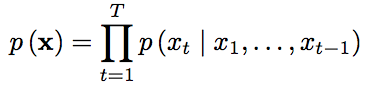
\includegraphics[scale=.5]{figures/rumus3}}
        \caption{Probabilitas Gabungan}
		\label{rumus3}
\end{figure}
Oleh karena itu, setiap sampel audio Xt dikondisikan pada sampel pada semua langkah waktu sebelumnya. Bukankah ini terlihat mirip dengan model peramalan deret waktu, di mana pengamatan pada langkah waktu bergantung pada pengamatan pada langkah waktu sebelumnya (Itulah yang kami coba modelkan menggunakan masing-masing istilah distribusi bersyarat ini)? Faktanya, WaveNet adalah model autoregresif.
Bagaimana kita melanjutkan untuk memodelkan istilah distribusi bersyarat ini? RNN atau LSTM menjadi model sekuensial non-linier yang kuat adalah pilihan yang paling jelas. Sebenarnya, Pixel RNN menggunakan ide yang sama untuk menghasilkan gambar sintetis yang terlihat mirip dengan gambar input. Bisakah kita menggunakan ide ini untuk menghasilkan pidato sintetis? Pidato sampel pada frekuensi minimal 16KHz, yang berarti bahwa setidaknya ada 16.000 sampel dalam satu detik pidato. RNN atau LSTM tidak akan dapat memodelkan dependensi waktu yang begitu lama (dari pesanan ~ 10.000 langkah waktu) karena mereka dapat memodelkan dependensi waktu paling banyak dari urutan 100 langkah waktu dan dengan demikian mereka tidak cocok untuk diucapkan perpaduan. Selain itu, melatih RNN, LSTM akan sangat lambat karena tidak dapat diparalelkan karena sifatnya yang berurutan secara inheren.Bisakah kita menggunakan CNN untuk menangani ini? Tunggu, CNN? Bagaimana? Mirip dengan ide yang telah digunakan di Pixel CNN.

\section{CNN}
Mengapa mencoba CNN? CNN biasanya lebih cepat untuk dilatih dibandingkan dengan RNN atau LSTM, terutama bila diterapkan pada urutan 1-D yang panjang karena operasi yang terkait dengan setiap posisi topeng atau filter yang berbelit-belit dapat dilakukan secara paralel dan independen. Pelatihan lebih cepat. Kedengarannya bagus! Bagaimana dengan properti autoregressive (output dari time-step bergantung pada output dari time-step sebelumnya saja dan bukan pada output dari time-steps di masa depan)? Di situlah Konvolusi Kausal beraksi. Konvolusi Kausal 1-D dapat dengan mudah diimplementasikan dengan mengisi ke kiri urutan input 1-D, di mana konvolusi akan dilakukan, dengan jumlah nol yang sesuai dan kemudian melakukan konvolusi yang valid.Causal Convolutions akan memungkinkan kita untuk memodelkan lebih lama (memungkinkan kita untuk menentukan panjang look-back juga) dependensi waktu dibandingkan dengan RNN atau LSTM.

\begin{figure}[H]
        \centerline{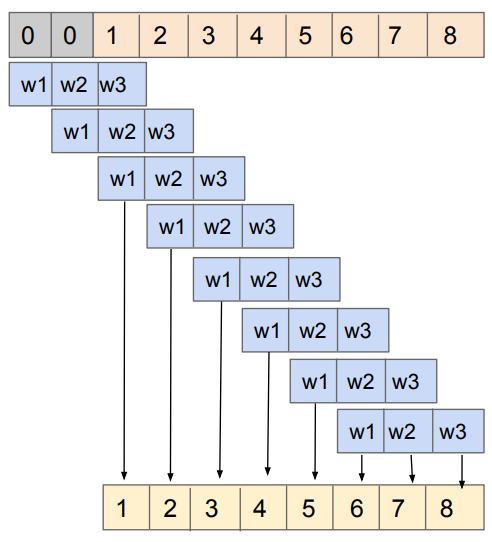
\includegraphics[scale=.5]{figures/cnn}}
        \caption{Konvolusi Kausal untuk memastikan bahwa model tidak dapat melanggar urutan di mana kita memodelkan data.}
		\label{cnn}
\end{figure}

Kita telah menangani pelanggaran autoregressive dengan mudah. Tetapi bagaimana dengan mengelola panjang lihat-belakang pesanan ribuan sampel (sehingga model kami melihat kembali setidaknya satu detik audio sebelum menarik kesimpulan tentang output pada langkah waktu saat ini)? Hal termudah yang terlintas dalam pikiran adalah meningkatkan ukuran filter yang cukup untuk melihat ke belakang dengan panjang yang sesuai, tetapi apakah ini benar-benar membantu? Dalam pandangan saya, melakukan hal itu akan membuat model kurang non-linier yang pada gilirannya akan mempersulit model kita untuk mempelajari dependensi temporal yang kompleks dan dengan demikian membatasi kinerja model kita. Hal berikutnya yang mungkin muncul di benak Anda adalah menambah jumlah lapisan dalam jaringan saraf. Ini mungkin membantu. Tapi itu akan menjadi komputasi yang tidak layak karena ukuran bidang reseptif atau melihat ke belakang untuk langkah waktu dalam output meningkat secara linier dengan jumlah lapisan tersembunyi dalam model dan tidak bijaksana secara komputasi bagi kita untuk memiliki model dengan beberapa ribu lapisan tersembunyi. Sekarang kita dibatasi untuk membatasi jumlah lapisan tersembunyi serta ukuran filter namun meningkatkan panjang tampilan kembali? Bagaimana kita akan melakukan ini? Konvolusi yang melebar akan membantu kita di sini. Sekarang kita dibatasi untuk membatasi jumlah lapisan tersembunyi serta ukuran filter namun meningkatkan panjang tampilan kembali? Bagaimana kita akan melakukan ini? Konvolusi yang melebar akan membantu kita di sini. Sekarang kita dibatasi untuk membatasi jumlah lapisan tersembunyi serta ukuran filter namun meningkatkan panjang tampilan kembali? Bagaimana kita akan melakukan ini? Konvolusi yang melebar akan membantu kita di sini.

Konvolusi melebar mencoba meningkatkan panjang tampilan atau ukuran bidang reseptif dengan menerapkan filter pada area yang lebih besar dari panjangnya dan melewatkan nilai input dengan langkah tertentu . Ini setara dengan konvolusi dengan filter yang lebih besar yang berasal dari filter asli dengan melebarkannya dengan nol tetapi secara signifikan lebih efisien. Di WaveNet, beberapa lapisan konvolusi melebar ditumpuk satu sama lain untuk memiliki bidang reseptif yang sangat besar hanya dengan beberapa lapisan. Peningkatan eksponensial (dua kali lipat) faktor pelebaran menghasilkan pertumbuhan bidang reseptif eksponensial dengan kedalaman.

\begin{figure}[H]
        \centerline{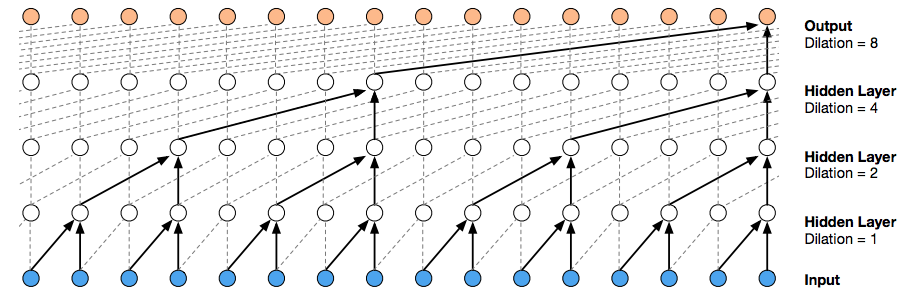
\includegraphics[scale=.35]{figures/cnn1}}
        \caption{Tumpukan lapisan konvolusi kausal yang melebar: Menggandakan faktor pelebaran dengan setiap lapisan menghasilkan pertumbuhan bidang reseptif O(2\^n).}
		\label{cnn1}
\end{figure}

\section{Softmax Distribution. Mu-law Companding}
Untuk memodelkan probabilitas bersyarat, WaveNet menggunakan distribusi softmax (kategorikal) daripada model campuran lainnya karena distribusi kategoris lebih fleksibel dan dapat lebih mudah memodelkan distribusi arbitrer karena tidak membuat asumsi tentang bentuknya.Audio mentah biasanya disimpan sebagai urutan nilai integer 16-bit (-32,768 hingga 32,767) dan menggunakan lapisan softmax untuk menampilkan distribusi probabilitas akan mengharuskan model kami untuk menghasilkan 65.535 nilai pada setiap langkah waktu. Bukankah ini akan memperlambat model kita? Itu pasti akan berhasil. Apa yang bisa kita lakukan tentang ini? Mengurangi kedalaman bit akan berhasil di sini. Jika kita terus menggunakan kedalaman bit linier (dibagi dengan 256) pengurangan akan memiliki dampak yang lebih besar pada sampel dengan amplitudo rendah daripada pada sampel dengan amplitudo tinggi. Pertimbangkan sampel 16-bit yang awalnya 32767, nilai positif tertinggi yang mungkin. Dikonversi menjadi 8 bit, nilai sampel menjadi 127 (32767/256 = 127 dengan sisa 255) dan error dari pembulatan adalah 255/32768. Ini adalah kesalahan kuantisasi kurang dari 1\%. Tetapi bandingkan ini dengan kesalahan untuk sampel 16-bit dengan magnitudo terendah, antara 0 dan 255.Intinya adalah bahwa dengan metode pengurangan kedalaman bit linier, pembulatan ke bawah memiliki dampak yang lebih besar pada sampel dengan amplitudo rendah daripada pada sampel dengan amplitudo tinggi. Jika kita dapat mendistribusikan kembali nilai sampel sehingga ada lebih banyak level kuantisasi pada amplitudo yang lebih rendah dan lebih sedikit level kuantisasi pada amplitudo yang lebih tinggi, kesalahan kuantisasi ini dapat dikurangi. Itu sebabnya, alih-alih menggunakan kuantisasi linier sederhana, pengomposisian Mu-law (kuantisasi non-linier) telah digunakan di WaveNet.

\begin{figure}[H]
        \centerline{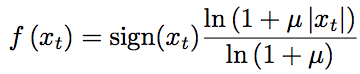
\includegraphics[scale=.5]{figures/rumus4}}
        \caption{Ekspresi untuk melakukan kompilasi Mu-law menghasilkan output yang direkonstruksi lebih baik (terdengar mirip dengan audio asli) daripada kuantisasi linier.}
		\label{rumus4}
\end{figure}

Dalam ekspresi di atas, 1 < Xt < 1 (pengambilan sampel audio pada langkah waktu yang berbeda disampel ulang dari 32,768…32,767 hingga 1…1) dan = 255. Ini akan membuat model hanya menghasilkan 256 nilai, bukan 65,535 nilai pada setiap langkah waktu, mempercepat pelatihan dan inferensi.

\section{Gated Activations. Skip and Residual Connections.}
Fungsi aktivasi non-linier sangat penting dalam setiap model pembelajaran mendalam untuk mempelajari hubungan kompleks antara output dan input. RELU awalnya digunakan di WaveNet, tetapi setelah melakukan eksperimen, disadari bahwa non-linearitas tan-hiperbolik gated dengan aktivasi sigmoid (terinspirasi dari Pixel CNN) bekerja lebih baik untuk WaveNet.
\begin{figure}[H]
        \centerline{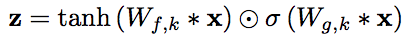
\includegraphics[scale=.5]{figures/rumus5}}
        \caption{Ekspresi untuk fungsi aktivasi terjaga keamanannya digunakan di WaveNet.}
		\label{rumus5}
\end{figure}
Dalam ekspresi di atas, W mewakili filter yang dapat dipelajari, * mewakili operator konvolusi dan titik yang dilingkari mewakili perkalian elemen-bijaksana. Koneksi sisa, menambahkan output dari lapisan bawah ke output dari lapisan di atas, dan Lewati koneksi, menambahkan output dari lapisan bawah langsung ke lapisan output, telah terbukti berguna dalam mengurangi waktu konvergensi jaringan saraf dan melatih jaringan yang lebih dalam. . Dengan demikian, mereka telah digunakan dalam arsitektur WaveNet, seperti yang ditunjukkan pada gambar di bawah ini.
\begin{figure}[H]
        \centerline{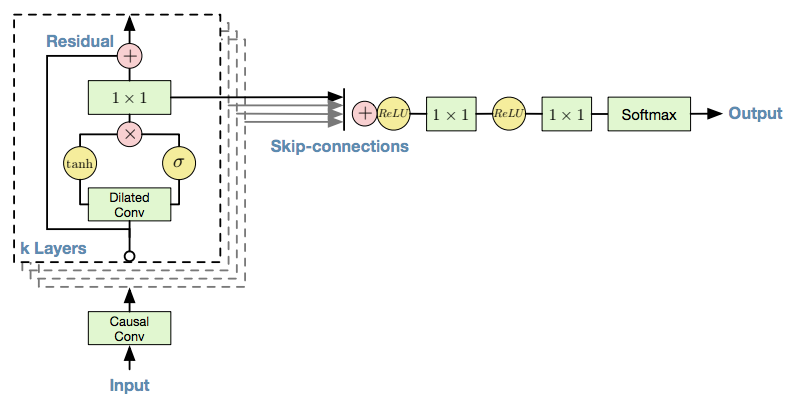
\includegraphics[scale=.35]{figures/rumus6}}
        \caption{Arsitektur WaveNet: menampilkan fungsi aktivasi yang terjaga keamanannya, melewatkan koneksi dan koneksi residual.}
		\label{rumus6}
\end{figure}

\section{Conditioning. Local. Global.}
Kami belum berbicara tentang bagaimana kami mengkondisikan ucapan keluaran berdasarkan berbagai fitur seperti identitas pembicara, teks yang sesuai, dll. Suara keluaran WaveNet dapat dikondisikan dalam dua cara: Pengkondisian global, keluaran bias fitur tunggal dari semua langkah waktu seperti identitas pembicara atau pengkondisian lokal, memiliki banyak fitur, pada kenyataannya serangkaian fitur waktu yang berbeda, yang membiaskan keluaran pada langkah waktu yang berbeda seperti teks yang mendasari pidato. Jika kita mengungkapkan ini secara lebih formal, maka ini berarti pengenalan parameter baru dalam istilah distribusi bersyarat ( Ht dalam pengkondisian lokal dan H dalam pengkondisian global) dalam model yang sebenarnya.
\begin{figure}[H]
        \centerline{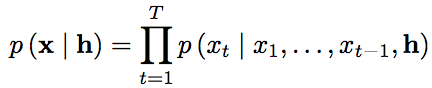
\includegraphics[scale=.5]{figures/rumus7}}
        \caption{Modifikasi istilah distribusi bersyarat, setelah pengenalan input pengkondisian.}
		\label{rumus7}
\end{figure}
Dalam pengkondisian lokal, kemungkinan rangkaian waktu input pengkondisian mungkin memiliki panjang yang lebih rendah daripada audio dan untuk pengkondisian lokal, kedua rangkaian waktu harus memiliki panjang yang sama. Untuk mencocokkan panjangnya, kita dapat menggunakan CNN yang ditransposisikan (semacam skema upsampling yang dapat dipelajari) atau skema upsampling lainnya untuk menambah panjang input pengkondisian.
\begin{figure}[H]
        \centerline{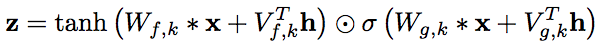
\includegraphics[scale=.5]{figures/rumus8}}
        \caption{Ekspresi setelah pengenalan istilah bias h.}
		\label{rumus8}
\end{figure}
Dalam ekspresi di atas, V adalah proyeksi linier yang dapat dipelajari yang pada dasarnya melayani dua tujuan mengubah h ke ukuran yang benar dan mempelajari bobot yang benar untuk bias output.

\section{Great Model. Fast Training. Slow Inference?}
Arsitektur WaveNet, apa pun yang telah kita bicarakan sampai sekarang, menangkap ketergantungan dan pengkondisian temporal yang kompleks dengan sangat baik. Selain itu, karena sangat dapat diparalelkan, ini sangat cepat pada waktu pelatihan. Tapi bagaimana dengan kesimpulannya? Karena output pada langkah waktu bergantung pada output pada langkah waktu sebelumnya, pengambilan sampel audio baru akan secara inheren berurutan. Butuh sekitar 1 menit waktu GPU untuk menghasilkan 1 detik output. Jika Google akan menerapkan model ini di Asisten mereka, maka akan memakan waktu berjam-jam untuk memikirkan pertanyaan sederhana seperti “Hai Google! Bagaimana cuacanya?”. Bagaimana mereka meningkatkan waktu inferensi? IAF adalah jawabannya.

\section{Normalising Flows. IAF.}
Normalisasi aliran? Aliran normalisasi adalah urutan transformasi yang mempelajari pemetaan (bijeksi) dari kepadatan probabilitas sederhana (seperti Gauss) menjadi distribusi kompleks yang kaya. Misalkan Anda memiliki cukup titik sampel dari distribusi probabilitas q(z) dan distribusi probabilitas q(x) , maka aliran normalisasi dapat digunakan untuk mempelajari transformasi yang akan memetakan titik sampel dari q(x) ke pemetaan yang sesuai dalam distribusi q (z) . Bagaimana ini dilakukan? Mari kita pertimbangkan transformasi f , pemetaan yang dapat dibalik dan halus. Jika kita menggunakan pemetaan ini untuk mengubah variabel acak z dengan distribusi q(z), variabel acak yang dihasilkan z' = f(z) memiliki distribusi q(z') :

\begin{figure}[H]
        \centerline{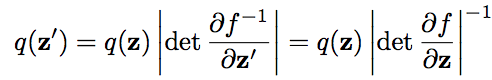
\includegraphics[scale=.5]{figures/rumus9}}
		\label{rumus9}
\end{figure}

Untuk mendapatkan intuisi tentang bagaimana kami mencapai ekspresi ini untuk distribusi variabel acak yang ditransformasikan, lihat posting blog ini oleh Eric Jang. Apakah satu transformasi f cukup? Faktanya, kita dapat membangun kepadatan kompleks yang sewenang-wenang dengan menyusun beberapa transformasi sederhana dan secara berturut-turut menerapkan ekspresi di atas. Kerapatan qK(z) yang diperoleh dengan mentransformasikan variabel acak z0 secara berurutan dengan distribusi q0 melalui rantai transformasi K fk adalah:

\begin{figure}[H]
        \centerline{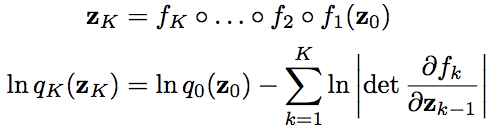
\includegraphics[scale=.5]{figures/rumus10}}
		\label{rumus10}
\end{figure}

Masing-masing transformasi ini dapat dengan mudah dimodelkan menggunakan perkalian matriks (dengan nilai yang dapat dipelajari), diikuti oleh non-linier seperti ReLU. Idenya kemudian adalah memperbarui parameter transformasi yang dapat dipelajari, dengan salah satu algoritme pengoptimalan favorit Anda dengan mengoptimalkan kemungkinan (log-likelihood) titik sampel dari q(x) di bawah distribusi probabilitas yang ditransformasikan qK(z). Ini akan membuat distribusi qK(z) sangat mirip dengan q(x) , dan dengan demikian mempelajari pemetaan yang sesuai dari q(z) ke q(x) .

\begin{figure}[H]
        \centerline{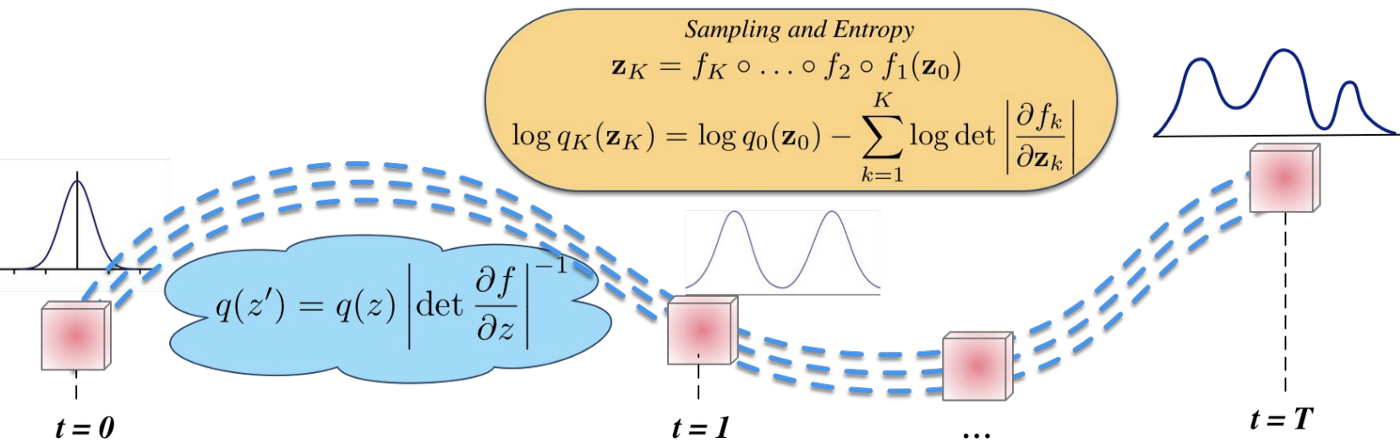
\includegraphics[scale=.25]{figures/rumus11}}
        \caption{Distribusi mengalir melalui urutan transformasi yang dapat dibalik.}
		\label{rumus11}
\end{figure}
Bagaimana ide normalisasi aliran dapat membantu kita dalam inferensi cepat? Ingat, WaveNet menjadi model generatif, tidak melakukan apa-apa selain mencoba mempelajari distribusi probabilitas yang akan menghasilkan data pelatihan dan karena ini adalah model generatif yang didefinisikan secara eksplisit (dengan kepadatan yang dapat dilacak), kita dapat dengan mudah mempelajari transformasi yang dapat memetakan titik dari titik sederhana. distribusi seperti Gaussian ke distribusi Kategoris kompleks yang dipelajari oleh WaveNet. Jika aliran normalisasi yang dipelajari yang memiliki skema inferensi cepat, masalah inferensi lambat kita di WaveNet dapat dengan mudah diurutkan. IAF (Inverse Autoregressive Flow) sangat cocok dengan ide ini.
Di IAF, idenya adalah pertama-tama menggambar sampel acak dari z Logistic (0, I) dan kemudian menerapkan transformasi berikut ke sampel yang diambil,
\begin{figure}[H]
        \centerline{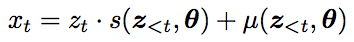
\includegraphics[scale=.5]{figures/rumus12}}
        \caption{Transformasi skala dan pergeseran sederhana pada zt di mana faktor penskalaan (s) dan faktor pergeseran (µ) dihitung dengan menggunakan parameter yang dapat dipelajari dan nilai dalam sampel input z dari langkah waktu sebelumnya.}
		\label{rumus12}
\end{figure}
Untuk menampilkan distribusi yang benar untuk langkah waktu xt , aliran autoregresif terbalik dapat secara implisit menyimpulkan apa yang akan dihasilkannya pada langkah waktu sebelumnya x1, . . . , xt-1 berdasarkan input noise z1, . . . , zt-1 , yang memungkinkan untuk menampilkan semua xt secara paralel diberikan zt . Gambar di bawah akan membuat segalanya lebih jelas (perhatikan notasi yang diubah).
\begin{figure}[H]
        \centerline{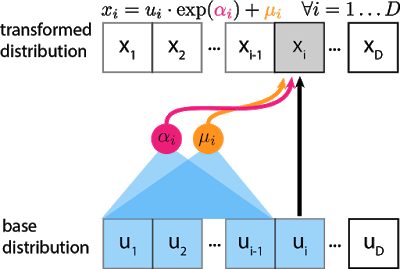
\includegraphics[scale=.5]{figures/rumus13}}
        \caption{Dalam Inverse Autoregressive Flow, output pada langkah waktu yang berbeda dapat dihitung secara paralel karena output dari langkah waktu tidak bergantung pada output dari langkah waktu sebelumnya.}
		\label{rumus13}
\end{figure}
IAF memiliki skema inferensi yang cepat (dan bahkan probabilitas bersyarat yang dapat dilacak dapat dihitung secara paralel), tetapi mereka lebih lambat untuk dilatih. Mengapa? Karena jika Anda jika kami diberi titik data baru dan diminta untuk mengevaluasi kepadatan, kami perlu memulihkan Anda dan proses ini secara inheren berurutan lambat. Paralel WaveNet, memanfaatkan fakta ini dan muncul dengan konsep pelatihan IAF (Student WaveNet) menggunakan WaveNet sederhana (Guru WaveNet).

\section{Parallel. Faster. WaveNet.}
Di WaveNet paralel, idenya adalah untuk memanfaatkan fakta bahwa IAF memiliki skema inferensi cepat. Jadi, pada fase pertama kami melatih model WaveNet sederhana (yang kami sebut sebagai Pelatihan Guru). Pada fase kedua, kami membekukan bobot Teacher WaveNet dan menggunakannya untuk melatih IAF (Student Distillation). Idenya adalah pertama-tama mengambil sampel acak dari z Logistic(0, I), melewatinya melalui IAF secara paralel. Ini akan memberi kita titik dalam distribusi yang ditransformasikan dan probabilitas bersyarat yang terkait juga. Idenya adalah untuk melewati titik ini dalam distribusi yang ditransformasikan di seluruh Teacher WaveNet sederhana, yang akan menghasilkan probabilitas bersyarat sehubungan dengan Teacher WaveNet yang sudah terlatih. Kemudian kami mencoba untuk meminimalkan perbedaan KL antara probabilitas bersyarat yang diterima dari kedua model. Ini akan memungkinkan IAF (Student WaveNet) untuk mempelajari distribusi probabilitas yang hampir sama dengan pengajarnya, dan hasil memvalidasi fakta ini karena ada perbedaan yang hampir dapat diabaikan dalam skor MOS skala 5 antara keluaran yang diterima dari WaveNet Guru dan Siswa.

\begin{figure}[H]
        \centerline{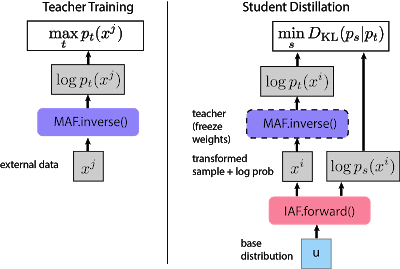
\includegraphics[scale=.5]{figures/rumus14}}
        \caption{Prosedur pelatihan Paralel WaveNet.}
		\label{rumus14}
\end{figure}

Apakah ini cukup cepat untuk disebarkan? Ya itu. Bahkan, ia mampu menghasilkan sampel ucapan lebih dari 20 kali lebih cepat daripada waktu nyata. Namun masih ada masalah, setiap kali kita perlu melatih kembali model kita, pertama-tama kita akan melatih WaveNet Guru dan kemudian WaveNet Siswa. Selain itu, kinerja Student WaveNet sangat bergantung pada seberapa baik Teacher WaveNet dilatih. Tapi secara keseluruhan bagus untuk pergi ke penyebaran.